\chapter{Simetría de intercambio, espín y los dos signos menos}

\section{Llenado de capas y la cuestión de las estadísticas del espín--}

La revisión del modelo de capas comienza con dos propiedades asociadas a los electrones. El electrón tiene espín un medio, con las dos proyecciones de espín adimensionales
\begin{equation}
m_s=+\frac12,
\qquad
m_s=-\frac12,
\end{equation}
y los electrones obedecen el principio de exclusión de Pauli. Estos hechos están relacionados, pero no son la misma afirmación.

La expresión ``el mismo estado'' requiere precisión. Ningún par de electrones puede ocupar el mismo estado completo de una partícula. Sin embargo, dos electrones pueden compartir un orbital espacial si sus estados de espín son distintos. En la aproximación de electrones independientes para el helio, ambos electrones ocupan el orbital espacial más bajo, uno con espín hacia arriba y el otro con espín hacia abajo. Más precisamente, las alternativas ``el primero tiene espín hacia arriba y el segundo, hacia abajo'' y ``el primero tiene espín hacia abajo y el segundo, hacia arriba'' pertenecen a un estado de espín entrelazado de dos electrones.

Esta es solo la antigua aproximación del modelo de capas. Ignora la interacción entre los electrones y se usa aquí por su sencillez para contar. En el litio, los dos primeros electrones llenan el orbital espacial más bajo con espines opuestos. El tercero no puede ocupar ninguno de esos estados completos y debe ocupar un orbital de mayor energía.

El siguiente paso es el conocido diagrama del momento angular orbital. Los sectores con
\begin{equation}
\ell=0,\qquad \ell=1,\qquad \ell=2
\end{equation}
se llaman estados \(S\), \(P\) y \(D\). Para un valor fijo de \(\ell\) hay
\begin{equation}
2\ell+1
\end{equation}
estados orbitales, de modo que
\begin{equation}
\ell=0\Rightarrow 1,
\qquad
\ell=1\Rightarrow 3,
\qquad
\ell=2\Rightarrow 5.
\end{equation}
El problema de Coulomb tiene degeneraciones adicionales: niveles radiales de distintos sectores de \(\ell\) pueden tener la misma energía. Para el argumento sobre el llenado de capas, la siguiente capa contiene un orbital \(S\) y tres orbitales \(P\). Por tanto, tiene
\begin{equation}
1+3=4
\end{equation}
estados espaciales. El espín duplica el número:
\begin{equation}
2(1+3)=8.
\end{equation}

Esos ocho estados completos de una partícula se llenan en la progresión sencilla desde el litio hasta el neón. Más allá de la capa cerrada, el sodio vuelve a tener un electrón exterior, por lo que esta imagen rudimentaria hace que se parezca al litio. La química no es el objetivo. Lo importante es que el espín semientero y la exclusión aparecen juntos.

Los fotones ofrecen el contraste. Tienen espín entero y no obedecen una regla de exclusión. Una onda electromagnética clásica corresponde a muchos fotones que ocupan el mismo modo. Los bosones pueden acumularse en un estado común, mientras que los fermiones idénticos no pueden ocupar más de una vez un mismo estado completo. La pregunta es si esas dos asociaciones podrían haber sido distintas: espín semientero sin exclusión o espín entero con exclusión. En tres dimensiones espaciales, la relación entre espín-- y estadística dice que no. La afirmación conocida requiere matices en una y dos dimensiones espaciales, y aquí no se intenta demostrar el resultado de la teoría de campos.

\begin{classroomqa}
\lecturetimestamp{00:11:48}
\audiencequestion{¿Existe un número máximo de cuantos bosónicos que puedan ocupar un estado?}
\lecturerresponse{No. Los bosones no tienen límite de ocupación y tienden a acumularse en el mismo estado.}
\end{classroomqa}

\section{Funciones de onda de muchas partículas}

Abordaremos la conexión mediante dos signos menos: uno proviene del intercambio y el otro de la rotación. Empecemos por el intercambio y, por el momento, dejemos de lado el espín.

Sea \(x_i\) la posición de la partícula \(i\). El subíndice identifica a la partícula; no es una componente cartesiana. Las tres coordenadas espaciales se condensan en el símbolo \(x_i\). Una base de posiciones para \(n\) partículas es
\begin{equation}
\lvert x_1,x_2,\ldots,x_n\rangle.
\end{equation}
Para un estado abstracto \(\lvert\Psi\rangle\), la función de onda en coordenadas es
\begin{equation}
\psi(x_1,x_2,\ldots,x_n)
=
\langle x_1,x_2,\ldots,x_n\mid\Psi\rangle.
\end{equation}
Su módulo al cuadrado,
\begin{equation}
\bigl\lvert\psi(x_1,x_2,\ldots,x_n)\bigr\rvert^2,
\end{equation}
es la densidad de probabilidad conjunta de encontrar la partícula \(1\) en \(x_1\), la partícula \(2\) en \(x_2\), y así sucesivamente.

Supongamos ahora que las partículas son idénticas. Imaginemos primero que pintamos de azul un electrón y de rojo otro. Entonces ``\(x_1\)azul en \(x_2\)''`` podría distinguirse de \(x_2\)azul en \(x_1\)''. Los electrones reales no llevan esos colores ni etiquetas individuales. Intercambiar las etiquetas que usamos para llevar la cuenta no puede crear una nueva configuración física.

Una fase global no cambia las probabilidades ni los valores esperados. Por tanto, para un estado perteneciente a un sector de intercambio definido, la función de onda en coordenadas puede satisfacer
\begin{equation}
\psi(x_2,x_1)=\eta\,\psi(x_1,x_2),
\qquad
\lvert\eta\rvert=1.
\end{equation}
Aplicar dos veces el mismo intercambio devuelve los argumentos originales y da
\begin{equation}
\eta^2=1,
\end{equation}
Así, los dos valores propios posibles para el intercambio son
\begin{equation}
\eta=+1
\qquad\hbox{or}\qquad
\eta=-1.
\end{equation}

\editorialnote{El álgebra del doble intercambio determina los valores propios posibles solo después de suponer que el estado tiene un comportamiento de intercambio definido. La restricción adicional de que los estados permitidos de una especie dada pertenezcan a un único sector de intercambio es una regla física; no se deduce de \(\eta^2=1\) por sí sola. La misma precisión se aplica al argumento de exclusión que sigue: la antisimetría implica exclusión una vez seleccionado el sector fermiónico, pero el álgebra del intercambio por sí sola no selecciona ese sector.}

Para los bosones, las funciones de onda permitidas son simétricas,
\begin{equation}
\psi_B(x_1,x_2)=\psi_B(x_2,x_1),
\end{equation}
mientras que para los fermiones son antisimétricas,
\begin{equation}
\psi_F(x_1,x_2)=-\psi_F(x_2,x_1).
\end{equation}
El signo menos no se aprecia cuando multiplica el estado entero, pero sí importa al sumar amplitudes. Así es como la simetría de intercambio adquiere consecuencias observables.

\section{Productos, sumas y exclusión}

Consideremos primero dos partículas asignadas al mismo orbital de una partícula \(\psi_0\). Su producto es
\begin{equation}
\psi_0(x_1)\psi_0(x_2).
\end{equation}
Al intercambiar las coordenadas de las partículas se obtiene
\begin{equation}
\psi_0(x_2)\psi_0(x_1)
=
\psi_0(x_1)\psi_0(x_2).
\end{equation}
Los valores de la función de onda son números, no operadores, así que los factores conmutan. El producto para el mismo estado es simétrico. Es una forma permitida para los bosones, pero no puede describir dos fermiones idénticos.

Asignemos ahora las partículas a orbitales distintos de una partícula:
\begin{equation}
\psi_0(x_1)\psi_1(x_2).
\end{equation}
El intercambio produce
\begin{equation}
\psi_0(x_2)\psi_1(x_1).
\end{equation}
Si las funciones son distintas, el producto intercambiado, en general, no es ni la expresión original ni su opuesta. Por tanto, el producto sin más no tiene ninguna de las simetrías de intercambio requeridas. Esto no impide que una partícula ocupe \(\psi_0\) mientras otra ocupa \(\psi_1\). Significa que el estado de dos partículas debe combinar las dos asignaciones.

La combinación simétrica es
\begin{equation}
\psi_B^{(01)}(x_1,x_2)
\propto
\psi_0(x_1)\psi_1(x_2)
+
\psi_0(x_2)\psi_1(x_1),
\end{equation}
y la combinación antisimétrica es
\begin{equation}
\psi_F^{(01)}(x_1,x_2)
\propto
\psi_0(x_1)\psi_1(x_2)
-
\psi_0(x_2)\psi_1(x_1).
\end{equation}
Los signos de proporcionalidad bastan, porque para el argumento sobre el intercambio no hace falta normalizar. Ambos estados contienen una partícula en cada orbital; solo difieren en cómo combinan las dos asignaciones indistinguibles.

Hagamos coincidir ahora los orbitales. La combinación bosónica se convierte en
\begin{align}
\psi_B^{(00)}(x_1,x_2)
&\propto
\psi_0(x_1)\psi_0(x_2)
+
\psi_0(x_2)\psi_0(x_1)\\
&=
2\psi_0(x_1)\psi_0(x_2),
\end{align}
que no es nula. La combinación fermiónica da
\begin{align}
\psi_F^{(00)}(x_1,x_2)
&\propto
\psi_0(x_1)\psi_0(x_2)
-
\psi_0(x_2)\psi_0(x_1)\\
&=0.
\end{align}
Con la regla de intercambio antisimétrica, se deduce la exclusión: no existe un estado antisimétrico no nulo en el que ambos fermiones estén en el mismo estado de una partícula.

Para un estado de muchas partículas, la regla se aplica a cualquier transposición de dos argumentos. Una transposición deja inalterada una función de onda bosónica y cambia el signo de una fermiónica. Repetir la misma transposición no produce ningún cambio en ninguno de los dos casos. Lo sorprendente es que un solo intercambio, aunque no cambie ninguna etiqueta observable de las partículas, cambia el signo de un estado fermiónico.

\section{El espín en la etiqueta completa de la partícula}

Ahora podemos reincorporar el espín con un pequeño cambio. La amplitud de una partícula depende tanto de la posición como de una etiqueta discreta de espín,
\begin{equation}
\psi(x,\sigma),
\end{equation}
donde \(\sigma=+1\) o \(-1\) indica el resultado elegido para \(\sigma_z\). El módulo al cuadrado es la densidad de probabilidad conjunta para la posición y la etiqueta de espín especificadas.

Para muchas partículas, la función de onda es
\begin{equation}
\psi(x_1,\sigma_1;\,x_2,\sigma_2;\,\ldots).
\end{equation}
El intercambio permuta todo lo que pertenece a las dos partículas, no solo sus posiciones:
\begin{align}
\psi_B(x_1,\sigma_1;\,x_2,\sigma_2)
&=
+\psi_B(x_2,\sigma_2;\,x_1,\sigma_1),\\
\psi_F(x_1,\sigma_1;\,x_2,\sigma_2)
&=
-\psi_F(x_2,\sigma_2;\,x_1,\sigma_1).
\end{align}
Esta es la formulación precisa de la afirmación inicial sobre el modelo de capas. Dos electrones pueden compartir un orbital espacial solo si sus estados completos, incluido el espín, son distintos.

\begin{classroomqa}
\lecturetimestamp{00:34:33}
\audiencequestion{¿Es la simetría de intercambio un caso particular del grupo de permutaciones?}
\lecturerresponse{Sí. Intercambiar partículas es una permutación, y la ley de transformación con signo más o menos da una representación del grupo de permutaciones.}
\end{classroomqa}

\begin{classroomqa}
\lecturetimestamp{00:35:12}
\audiencequestion{¿Por qué la construcción de dos partículas es un producto y no una suma de las funciones de onda de una partícula?}
\lecturerresponse{Una suma describe una partícula en una superposición. Un producto pertenece al espacio producto tensorial de dos partículas y describe una partícula asignada a cada estado de una partícula.}
\end{classroomqa}

El intercambio de las etiquetas completas se muestra en la pizarra de abajo.\footnote{El orden de las etiquetas de posición--espín se reconstruye a partir del fotograma legible de la pizarra y de la explicación circundante, desde 00:33:43 hasta 00:34:25.}
\begin{figure}[htbp]
\centering
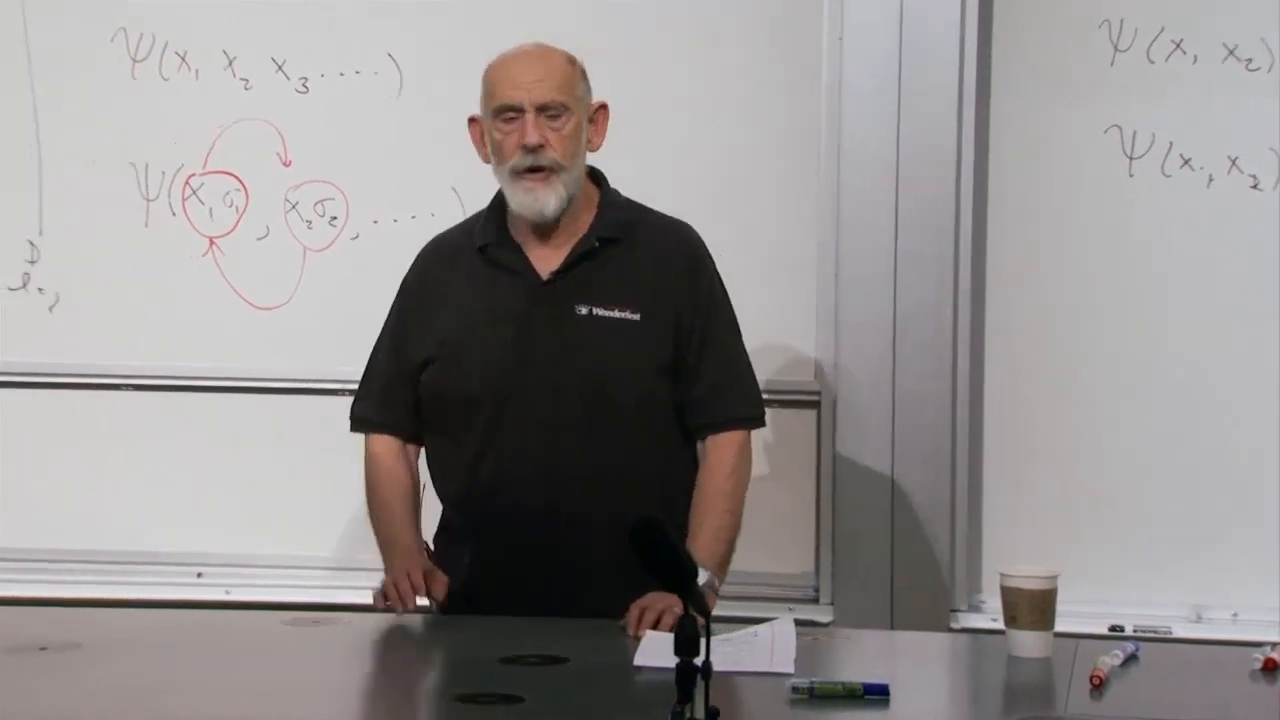
\includegraphics[width=0.9\linewidth]{lecture_05_frame_03.png}
\caption{Al intercambiar dos partículas idénticas se permutan sus etiquetas completas de posición--espín. Un estado bosónico permanece inalterado, mientras que uno fermiónico cambia de signo.}
\lectureframe{00:35:25}
\end{figure}

Estos son dos usos distintos de la linealidad. Para una partícula,
\begin{equation}
\alpha\psi_0(x)+\beta\psi_1(x)
\end{equation}
es una superposición de dos alternativas. Para dos partículas,
\begin{equation}
\psi_0(x_1)\psi_1(x_2)
\end{equation}
es una amplitud producto en un espacio con dos coordenadas de partícula. La simetrización o antisimetrización combina ese producto con su versión intercambiada.

\begin{classroomqa}
\lecturetimestamp{00:36:13}
\audiencequestion{¿El intercambio de partículas produce un efecto de interferencia?}
\lecturerresponse{Sí. La amplitud fermiónica nula para el mismo estado puede entenderse como interferencia destructiva entre las dos contribuciones intercambiadas.}
\end{classroomqa}

\begin{classroomqa}
\lecturetimestamp{00:37:13}
\audiencequestion{¿Derivó Pauli la exclusión mediante este mismo argumento de simetría?}
\lecturerresponse{Pauli partió de un hecho empírico y encontró un marco matemático en el que podía expresarse. Al principio no estaba derivando la exclusión de una teoría más fundamental.}
\end{classroomqa}

La antisimetría proporciona el marco matemático en el que se expresa la regla empírica de exclusión.

\begin{classroomqa}
\lecturetimestamp{00:39:01}
\audiencequestion{¿Está relacionada la interferencia por intercambio de partículas con la interferencia entre caminos alternativos?}
\lecturerresponse{Sí. En una historia, las dos partículas pasan sin cruzarse; en otra, se cruzan y llegan a los destinos intercambiados. Las amplitudes se suman para los bosones y pueden cancelarse para los fermiones.}
\end{classroomqa}

El intercambio aporta el primer signo menos. La rotación aporta el segundo.

\section{El segundo signo menos: rotación de \texorpdfstring{\(2\pi\)}{2 pi}}

Una rotación completa parece no producir ningún efecto. Toda dirección geométrica ordinaria vuelve a su posición inicial tras un ángulo de \(2\pi\). Sin embargo, lo que debe volver a sus valores iniciales son las probabilidades y los valores esperados. El propio vector de estado puede volver con una fase global, igual que puede hacerlo tras un intercambio.

\begin{classroomqa}
\lecturetimestamp{00:42:12}
\audiencequestion{¿Qué eje se usa para la rotación y cuál es el generador: el momento angular orbital, el espín o ambos?}
\lecturerresponse{Se puede elegir un eje externo; aquí tomaremos el eje \(z\). El generador es el momento angular total, que incluye las contribuciones orbital y de espín. El espín no tiene por qué apuntar a lo largo del eje elegido.}
\end{classroomqa}

\editorialnote{En esta discusión, las fórmulas del momento angular usan \(\hbar=1\), de modo que \(m\) es el valor propio adimensional de \(J_z\).}

Sea \(\psi(\theta)\) el estado obtenido al variar el parámetro de rotación a lo largo de un ángulo \(\theta\). Con la convención usada aquí,
\begin{equation}
J_z\psi(\theta)
=
-i\frac{\partial}{\partial\theta}\psi(\theta).
\end{equation}
Para un estado con \(J_z\) definido,
\begin{equation}
J_z\psi(\theta)=m\psi(\theta).
\end{equation}
Al combinar las ecuaciones se obtiene
\begin{equation}
-i\frac{\partial}{\partial\theta}\psi(\theta)
=
m\psi(\theta),
\end{equation}
cuya solución es
\begin{equation}
\psi(\theta)=e^{im\theta}\psi(0).
\end{equation}

Los valores permitidos de \(m\) son enteros o semienteros. Por tanto,
\begin{equation}
\psi(2\pi)
=
\begin{cases}
+\psi(0), & m\in\mathbb Z,\\[4pt]
-\psi(0), & m\in\mathbb Z+\tfrac12.
\end{cases}
\end{equation}
Tras otra vuelta completa,
\begin{equation}
\psi(4\pi)=\psi(0)
\end{equation}
en cualquiera de los dos casos. Este es el segundo signo menos: un estado de un multiplete de momento angular semientero cambia de signo bajo una rotación de \(2\pi\).

El signo no altera \(\lvert\psi\rvert^2\), así que no se aprecia cuando multiplica el estado entero. Aun así, una rotación de \(2\pi\) no está representada por la identidad en un estado de espín semientero. La diferencia se vuelve observable cuando el signo es relativo a otra amplitud coherente.

\section{Los caminos de \texorpdfstring{\(2\pi\) y \(4\pi\)}{2 pi y 4 pi}}

La diferencia entre \(2\pi\) y \(4\pi\) puede hacerse visible sin más álgebra. Sostén una taza con una mano y gírala una vuelta completa sin soltarla. La taza recupera su orientación original, pero el brazo queda retorcido. Continúa con una segunda vuelta y podrás devolver el brazo a su posición original sin invertir el movimiento de la taza.

Una construcción relacionada consiste en colocar una esfera dentro de una caja y unirla a la caja con cuerdas. Al girar la esfera \(2\pi\), las cuerdas quedan enredadas. En el espacio tridimensional ordinario, puede deshacerse el enredo asociado a un giro de \(4\pi\). El objeto pertinente no es simplemente la orientación final de la esfera, sino el camino recorrido por el espacio de rotaciones.

\begin{classroomqa}
\lecturetimestamp{00:54:22}
\audiencequestion{Si se gira la esfera dos veces alrededor del mismo eje, ¿se pueden desenredar realmente las cuerdas? ¿Hace falta otra dimensión espacial?}
\lecturerresponse{El camino de \(4\pi\) puede deshacerse en el espacio tridimensional ordinario. El tiempo parametriza el movimiento; no es otra dirección espacial. Un camino de \(2\pi\) no puede deshacerse de este modo, mientras que uno de \(4\pi\) sí puede.}
\end{classroomqa}

Las demostraciones distinguen un camino no trivial de \(2\pi\) de un camino deshacible de \(4\pi\), sin desarrollar una teoría formal del grupo de rotaciones.

\section{Intercambio y rotación en la imagen de la correa}

Ahora aparecen juntos los dos signos menos. Intercambiar dos fermiones idénticos cambia el signo de su función de onda conjunta. Girar un estado de espín semientero en \(2\pi\) también cambia su signo. Una correa establece una relación geométrica entre ambas operaciones.

Dispón la correa de modo que se hayan intercambiado sus dos extremos inferiores. Vista de otro modo, la misma correa tiene un giro de \(2\pi\). Al efectuar el intercambio junto con la rotación de \(2\pi\), se elimina el giro y la correa queda sin torsión. El proceso combinado puede reducirse continuamente a no hacer nada.\footnote{La observación sobre el intercambio--la rotación se atribuye a David Finkelstein en la conferencia. El registro de la fuente no identifica ninguna publicación concreta, por lo que aquí el nombre se conserva únicamente como parte de esa atribución.}

\begin{classroomqa}
\lecturetimestamp{01:01:12}
\audiencequestion{¿Se trata solo de cómo está incrustada la correa en el espacio, y no de una afirmación sobre la topología de las partículas?}
\lecturerresponse{La correa puede interpretarse como una historia de partículas en el espacio-tiempo. Si el tiempo avanza hacia arriba, una sección transversal muestra objetos parecidos a partículas. Se crean pares, se gira un objeto en \(2\pi\) y se intercambian dos objetos idénticos. En esa historia, las fases de rotación e intercambio se cancelan.}
\end{classroomqa}

La historia hace explícito el cómputo de las fases. Empecemos sin partículas. En dos lugares separados, creemos un par partícula--antipartícula, de modo que en un instante intermedio haya cuatro partículas. Giremos una partícula en \(2\pi\) mientras intercambiamos dos partículas idénticas en otro lugar de la configuración. La historia completa puede deformarse hasta la historia elemental en que se crea un par y luego se aniquila. En el cómputo de signos aquí considerado, esa historia trivial no tiene fase adicional. Si \(\eta_{\mathrm{rot}}\) y \(\eta_{\mathrm{ex}}\) representan los dos signos, la cancelación expuesta oralmente puede escribirse de forma compacta como sigue:\footnote{Esta ecuación de fase expresa la cancelación descrita desde 01:06:50 hasta 01:07:18; la conferencia presenta la construcción como sugerente, no como una demostración rigurosa.}
\begin{equation}
\eta_{\mathrm{rot}}\eta_{\mathrm{ex}}=1.
\end{equation}

\begin{classroomqa}
\lecturetimestamp{01:03:34}
\audiencequestion{¿Puede relacionarse el intercambio con las rotaciones haciendo que cada una de dos partículas gire \(\pi\) y luego reorientándolas?}
\lecturerresponse{Esa construcción quizá refleje matemáticas relacionadas, pero utiliza dos rotaciones separadas de \(\pi\). El proceso que analizamos aquí contiene una rotación de \(2\pi\), así que los dos argumentos no son idénticos.}
\end{classroomqa}

El argumento depende de que sea posible crear y aniquilar objetos parecidos a partículas. No tendría esta forma en una teoría en la que las partículas fueran eternas. Tampoco se presenta como la demostración habitual del teorema de espín--estadística. Su propósito es mostrar una razón topológica por la que los signos de intercambio y rotación concuerdan.

\section{Bultos, imágenes especulares y aniquilación}

La construcción puede repetirse con configuraciones localizadas de campos. Supongamos que uno o más campos adoptan sus valores de vacío casi en todas partes, pero presentan forma y estructura no nulas en una región pequeña. Esa configuración localizada es un bulto.

Construyamos ahora una segunda configuración que sea la imagen especular apropiada de la primera. Llamemos partícula a una y antipartícula a la otra. Acerquémoslas. Las partes correspondientes de las configuraciones de campo se encuentran y se deshacen mutuamente. En una etapa intermedia, algunas partes de los bultos pueden haber desaparecido mientras otras permanecen. Si continuamos la deformación, se elimina la estructura restante y los campos vuelven a la configuración de vacío. Dos torsiones opuestas en una correa dan la misma imagen: al empujarlas una hacia la otra, se deshacen.

El proceso puede recorrerse en sentido inverso. El espacio vacío puede producir un bulto y su compañero especular. Se pueden crear dos pares de este tipo, girar un bulto en \(2\pi\), intercambiar dos bultos idénticos y volver a aniquilar los pares. Se aplica entonces la misma cancelación entre intercambio--rotación. Esto sigue siendo una extensión heurística de la construcción, no un teorema sobre toda excitación localizada.

\begin{classroomqa}
\lecturetimestamp{01:11:30}
\audiencequestion{¿Existen realizaciones físicas de estas configuraciones de campo parecidas a bultos?}
\lecturerresponse{Sí. Algunos ejemplos son los núcleos en descripciones de tipo Skyrmion, los monopolos magnéticos y otras excitaciones de campos parecidas a partículas.}
\end{classroomqa}

La imagen de los bultos especulares permite entender la generalización. Lo pertinente no es que el objeto empezara como una partícula puntual elemental, sino que una excitación parecida a una partícula y su compañera puedan crearse, acercarse y aniquilarse de manera continua. Esa característica motiva una relación más amplia entre el comportamiento bajo rotación y bajo intercambio.

\begin{classroomqa}
\lecturetimestamp{01:16:12}
\audiencequestion{¿Significa espín un medio que el estado acumula solo la mitad de la fase de rotación habitual?}
\lecturerresponse{En esta convención, la fase es \(e^{im\theta}\). Para \(m\) semientero, una rotación de \(2\pi\) da \(-1\), mientras que una rotación de \(4\pi\) da \(+1\).}
\end{classroomqa}

\section{Un signo global y un experimento nulo}

¿Se puede observar el signo menos de una rotación de \(2\pi\)? Empecemos con un experimento en el que no se puede. Confinemos un electrón en un campo magnético, dejemos que su espín siga el campo mientras el aparato gira lentamente en \(2\pi\) y, a continuación, liberemos el electrón en un dispositivo de interferencia. Comparemos esto con el mismo procedimiento sin la rotación.

La rotación transforma el estado así:
\begin{equation}
\psi\longmapsto-\psi,
\end{equation}
pero el signo menos multiplica el estado entero. Todas las probabilidades permanecen iguales, por lo que el patrón de interferencia final no conserva ningún indicio de si tuvo lugar la rotación preliminar. Es un experimento nulo: una fase común no tiene con qué interferir.

\begin{classroomqa}
\lecturetimestamp{01:20:01}
\audiencequestion{¿Por qué debe hacerse lentamente la rotación del campo magnético?}
\lecturerresponse{El espín debe seguir acompañando al campo magnético giratorio. Si el campo se arrastra demasiado rápido, el espín no permanecerá alineado con él.}
\end{classroomqa}

\section{Un electrón en dos ramas coherentes}

El signo se vuelve observable cuando es relativo. Hagamos pasar un electrón por un divisor de haz. Una parte de su función de onda sigue un camino y otra parte sigue otro:
\begin{equation}
\psi(x)=\psi_1(x)+\psi_2(x).
\end{equation}
Es un electrón, no dos. Se encuentra en una superposición coherente de dos alternativas. Hay que tener clara la diferencia: los dos paquetes no son dos partículas independientes.

Guiemos los dos paquetes hacia regiones separadas que contienen campos magnéticos. Giremos el campo de una región en \(2\pi\), dejando el otro sin cambios. Para un estado de espín semientero,
\begin{equation}
\psi_1(x)+\psi_2(x)
\longmapsto
\psi_1(x)-\psi_2(x),
\end{equation}
donde la rama girada se ha etiquetado como \(2\). Ahora el signo es relativo. Cuando los dos paquetes vuelvan a superponerse, la suma se habrá convertido en resta. Un punto de interferencia constructiva puede convertirse en uno de interferencia destructiva, o incluso en un nodo.

\begin{classroomqa}
\lecturetimestamp{01:23:46}
\audiencequestion{¿Qué se está girando si hay un solo electrón pero dos ramas de la función de onda?}
\lecturerresponse{El electrón se encuentra en una superposición coherente de dos alternativas localizadas. Se gira una rama y la otra no. Si se abren las cajas para averiguar cuál de las alternativas ocurrió, esa medición destruye la interferencia.}
\end{classroomqa}

Abrir las cajas solo revelaría que hay un electrón, en una u otra caja. Sin esa medición, ambas amplitudes permanecen en el estado. Al repetir el experimento, el patrón de interferencia se forma detección a detección. En un nodo producido por el signo menos relativo no se detecta ningún electrón.

\section{Precesión magnética e interferencia de doble rendija}

Una disposición esquemática más práctica sustituye el experimento de las cajas, extremadamente lento. Dividamos una onda coherente de electrones en dos caminos. En uno de ellos, hagamos pasar el electrón por una región magnética con el espín inicialmente transversal al campo. Entonces el espín precesa. Al elegir la intensidad del campo y el tiempo de tránsito, se puede hacer que el espín de esa rama complete una vuelta de \(2\pi\), mientras que la otra rama no experimenta tal giro.\footnote{La conferencia afirma que se había realizado un experimento relacionado con la fase espinorial y describe su principio, pero el registro de la fuente no identifica ningún artículo ni aparato concreto. Por tanto, este relato se limita a la construcción presentada en la conferencia.}

\begin{classroomqa}
\lecturetimestamp{01:27:05}
\audiencequestion{¿Cómo se puede determinar el camino del electrón único?}
\lecturerresponse{No se puede determinar sin arruinar el experimento. Cualquier medición que registre qué camino siguió el electrón destruye la interferencia.}
\end{classroomqa}

\begin{classroomqa}
\lecturetimestamp{01:27:50}
\audiencequestion{¿Qué es exactamente una rama de la función de onda y cómo produce el divisor dos ramas?}
\lecturerresponse{Una rama es un paquete de ondas localizado a lo largo de un camino. El divisor transforma la onda incidente en dos paquetes separados espacialmente, y los campos eléctricos o magnéticos pueden guiarlos por caminos distintos.}
\end{classroomqa}

Salvo por la región magnética, este es el experimento de la doble rendija. Una onda electrónica incidente se separa en dos paquetes. Las ondas salientes se propagan hacia una región común de detección, donde sus amplitudes se superponen. Sin rotación relativa, las amplitudes centrales pueden sumarse. Una rotación de espín de \(2\pi\) en uno de los caminos invierte una amplitud y puede hacer que esas mismas contribuciones se cancelen.

\begin{classroomqa}
\lecturetimestamp{01:30:46}
\audiencequestion{¿Cómo puede haber interferencia si el electrón viaja por tubos o rendijas distintos?}
\lecturerresponse{La detección final no revela el camino. Las dos amplitudes de onda salientes se propagan y se superponen en el detector. Mirar para averiguar qué camino siguió destruiría la interferencia.}
\end{classroomqa}

\begin{classroomqa}
\lecturetimestamp{01:33:22}
\audiencequestion{¿Debe el diámetro del tubo o de la rendija ser comparable a la longitud de onda del electrón?}
\lecturerresponse{En una realización literal de doble rendija basada en la difracción, la abertura debe ser lo bastante pequeña para producir la dispersión necesaria. El aparato que se describe es esquemático, no un diseño práctico.}
\end{classroomqa}

\begin{classroomqa}
\lecturetimestamp{01:33:44}
\audiencequestion{¿Una rotación de la polarización de los fotones de \(2\pi\) dejaría inalterado el patrón de interferencia?}
\lecturerresponse{Sí. Los fotones tienen espín entero, por lo que una rotación completa de \(2\pi\) no introduce el signo menos fermiónico.}
\end{classroomqa}

\begin{classroomqa}
\lecturetimestamp{01:34:12}
\audiencequestion{¿En qué se aparta ligeramente el experimento práctico de la versión idealizada?}
\lecturerresponse{En el montaje ideal, el espín gira adiabáticamente. En la descripción práctica, el electrón atraviesa una región magnética y su espín precesa más rápidamente, pero la fase medida sigue siendo la asociada a un giro de \(2\pi\).}
\end{classroomqa}

El montaje lento aísla la idea al garantizar que el espín siga al campo sin movimiento adicional. El montaje con precesión produce dinámicamente el mismo signo relativo. En cualquiera de las dos versiones, las dos trayectorias deben dejar de ser distinguibles antes de que pueda aparecer un patrón de interferencia.

\begin{classroomqa}
\lecturetimestamp{01:36:15}
\audiencequestion{¿Es necesario recombinar las dos ramas después del divisor?}
\lecturerresponse{Sí. Los paquetes de ondas que emergen deben solaparse o extenderse sobre una región común de detección para que sus amplitudes puedan formar un patrón de interferencia.}
\end{classroomqa}

\begin{classroomqa}
\lecturetimestamp{01:38:12}
\audiencequestion{¿Es este experimento de rotación con un solo electrón una consecuencia del principio de exclusión de Pauli?}
\lecturerresponse{No. Solo hay un electrón. El experimento mide la fase del espinor bajo rotación, no la exclusión de dos fermiones de un mismo estado.}
\end{classroomqa}

\section{Interferencia por intercambio y rotación relativa}

El signo de intercambio podría ponerse de manifiesto mediante el mismo método general, aunque el aparato propuesto es más complicado. Se parte de dos electrones y se divide su función de onda conjunta en dos ramas coherentes. Siguen siendo solo dos electrones, no cuatro: el par sigue una alternativa o la otra. En una rama se intercambian los dos electrones y en la otra se dejan sin intercambiar. Cuando se vuelven a reunir las ramas, el signo de intercambio fermiónico aparece como una fase relativa y puede modificar la interferencia.

La propuesta final compara directamente los dos signos menos. Una rama adquiere la fase de intercambio fermiónica, mientras que la otra adquiere la fase correspondiente a una rotación de \(2\pi\). Ambas fases son \(-1\), por lo que el efecto relativo se cancela.\footnote{La grabación comprendida entre 01:40:26 y 01:41:15 muestra claramente una fase de intercambio, una fase de rotación de \(2\pi\) y su cancelación, pero no es posible recuperar del habla disponible la asignación detallada de la rotación.} La clase presenta esto como un experimento mental propuesto y afirma que, hasta donde sabe quien habla, no se había llevado a cabo.

\begin{classroomqa}
\lecturetimestamp{01:41:34}
\audiencequestion{¿Observar una fase de intercambio pondría en entredicho la indistinguibilidad de los dos electrones?}
\lecturerresponse{No. La indistinguibilidad cuántica es más sutil que la identidad clásica. Permite que el vector de estado cambie de signo bajo el intercambio, aunque ninguna etiqueta observable distinga las partículas.}
\end{classroomqa}

Queda una última salvedad. Si se rotara un mundo aislado entero en \(2\pi\), solo se obtendría una fase común, y ningún experimento interno podría revelarla. El experimento detectable rota una rama coherente con respecto a otra. Por tanto, lo que se observa no es un signo absoluto, sino la interferencia producida por un signo relativo.
